\documentclass{scrartcl}

\usepackage[backend=biber,style=apa,sorting=none]{biblatex}
\addbibresource{dd-v2.bib}
\let\cite\textcite
\let\citep\autocite
\usepackage{graphicx}
\graphicspath{{img/}}
\usepackage{hyperref}

% TODO list
% See issue https://github.com/summerysaturn/y1-university/issues/11
% [x] Working Title                 Done, Section 1.1
% [x] Concept Statement             Done, Section 1.2
% [x] Genre                         Done, Section 1.3
% [x] Target Audience               Done, Section 1.4
% [x] Unique Selling Points (USPs)  Done, Section 1.5
% [x] Player Experience             Done, Section 2.1
% [x] Visual and Audio style        Done, Section 2.2
% [x] Narrative (optional)          Done, Section 2.3
% [x] Platform and Technology       Done, Section 2.4
% [x] Game rules                    Done, Section 3.1
% [x] Core loops                    Done, Section 3.2
% [x] Control Schemes               Done, Section 3.3

\begin{document}
\author{Charlotte Ward}
\date{\today}
\title{
{\huge Working Title: Cybersky} \\
{\small A modern reimagining of classic Shoot 'em Up gameplay, designed for handheld play, featuring roguelite mechanics.} \\
{\small Genre: Roguelite, Shoot 'Em Up} \\
{\small Version 2.0.0}
}
\maketitle

\tableofcontents

\pagebreak

\section{
  High Level Design
 }

\subsection{Working Title}

The working title for this project is \emph{Cybersky}, using words linked to Science Fiction and dystopia settings.

\subsection{Concept Statement}

\begin{quote}
  \emph{A modern reimagining of classic Shoot 'em Up gameplay, designed for handheld play, featuring roguelite mechanics.}
\end{quote}

This statement quickly sums up the core of the game, demonstrating the historical basis that the Shoot 'em Up genre has. Additionally, the roguelite features and handheld nature are conveyed.

\subsection{Genre}

The genre of this game is described as a:

\begin{quote}
  \emph{Roguelite Shoot 'em Up (Shmup)}
\end{quote}

This description can be broken into two parts:

\subsubsection{Shoot 'em Up:}

The following subsection primarily follows an article by \cite{BrianW2020-01}.

Recent Shoot 'em Up games are an influence for \emph{Cybersky}, including \emph{'Ikaruga'}, a 2001 title that's often regarded as the epitome of \'Shmup\' design. \emph{Ikaruga} was very popular within the community of Shmups and Bullet Hells, quickly becoming the gold standard of the genre. In more recent years, \emph{'Enter the Gungeon'} has revitalised the Shmup genre, breathing some life back into the fandom.

Additionally, Shoot \'em Up games share ground with Twin-Stick Shooters, a specific subgenre that relates to a movement and combat system where one control stick controls movement, and another control stick affects firing direction. A notable example is \emph{'Geometry Wars: Retro Evolved 2'}.

The gameplay of a Shmup is designed around a large quantity of projectiles, involving player movement in the style to a Twin-Stick Shooter, or similar to a fixed shooter like \emph{Galaxian}. To summarise:

\begin{itemize}
  \item High quantity of projectiles \& enemies.
  \item Twin-Stick Shooter or Fixed Shooter movement.
\end{itemize}

\subsubsection{Roguelite:}

The following subsection primarily follows an article by \cite{BrianW2020-02}.

The genre of Roguelikes derive from the overall structure of the game \emph{'Rogue'}, a 1980 release, being the first implementation of the genre overall, bringing new conventions with it. These rules can be outlined as:

\begin{itemize}
  \item Permadeath
  \item Procedural generation
  \item Difficult enemies
  \item Loot based progression
\end{itemize}

Roguelike games implement these rules across many different genres, illustrating their versatility as a set of rules. A \emph{Roguelite} in particular is a subset of this genre, implementing some or all of these rules in a less strict or 'hardcore' way. This is particularly useful in describing \emph{Cybersky}, as the game should appeal to a more casual audience due to the target platform.

A few examples of Roguelike games include \emph{'Darkest Dungeon'} and \emph{'The Binding of Isaac'}. A more loose example of a Roguelite would be \emph{'FTL: Faster Than Light'}. These examples are good inspirations as they feature procedural generation and progression, and implement permadeath and loot-based progression.

\subsection{Target Audience}

With \emph{Ikaruga} being described as a "shooter-fan's shooter" by \cite{Rodriguez2018}, and the resulting success in the industry \citep{BrianW2020-01}, it's clear that \emph{Ikaruga} has become a bit of a cult classic, with few games reaching the same heights since. \emph{Cybersky} aims to appeal to the same fans that \emph{Ikaruga} had.

As well as this, \emph{Cybersky} is aimed at the general mobile market, meaning that it should follow the archetypical conventions of a mobile game: accessibility in terms of gameplay and design, simplicity, cognitive flow, short session length, all of which relate to the psychology and design trends in mobile gaming at the moment \citep{Northington2018}.

\subsubsection{Casual Persona}

This section is dedicated to the persona of a casual mobile gamer:

\begin{itemize}
  \item Name: Cynthia Enriquez
  \item Age: 27
  \item Gender: Female
  \item Job: Digital Marketing
\end{itemize}

Cynthia works full time as a digital marketing employee for a small company. She spends a lot of her time commuting by train to the small office and has little time to play games on a console or computer. She's looking for something easy to pick up and put down as her train journey has lots of stops. \emph{Cybersky} aims to fill this gap by being easily accessible for casual players, having short gameplay loops to help fill time in this kind of fractured manner.

\subsubsection{Fan Persona}

This section is dedicated to the persona of a fan of shmups:

\begin{itemize}
  \item Name: Jaylen Farrow
  \item Age: 22
  \item Gender: Male
  \item Job: Student
\end{itemize}

Jaylen is a student in university, spending a fair amount of time doing coursework and attending lectures. He uses a pomodoro timer to get work done effectively during the day, but needs a way to quickly unwind. He also is an enthusiast in the Bullet Hell genre and has been for many years, seeking out new games in the genre to deep-dive into and enjoy. \emph{Cybersky} aims to appeal to Jaylen by subscribing to the genre conventions, and has long-term progression alongside the short gameplay loop to allow for him to enjoy the game in this multifaceted way.

\subsection{Unique Selling Points}

This game aims to reintroduce classic Shoot 'em Up gameplay onto the mobile gaming market. With the industry tending towards monetisation and advertisement, there's a sore need for games that are simple and replayable. \emph{Cybersky} can achieve this by cutting past the annoying and often offputting monetisation that exists in mobile gaming, skipping advertisements and instead relying on a pay-what-you-want scheme.

To summarise:

\begin{itemize}
  \item Noninvasive Monetisation
  \item Pay what you want scheme
  \item Open source
\end{itemize}

Additionally, \emph{Cybersky} includes roguelite features, featuring short levels that make up part of a larger 'run' narrative. Each of these levels are chosen procedurally and have their own features, gimmicks and enemy/loot types. Players choose between an amount of paths forward, being told the general category that each path fits into.

While \emph{Cybersky} is permadeath for each 'run', there are permanent unlocks that can manipulate the way the game is played and add complexity depending on the amount the player has played the game.

To summarise:

\begin{itemize}
  \item 'Roguelite' features
  \item Revolves around 'runs'
  \item Choose your own adventure style progression
  \item Item synergy
  \item Progressive upgrades
  \item Pseudo-Permadeath
  \item Permanent unlocks
\end{itemize}

\section{
  Product Design
 }

\subsection{Player Experience}

The player controls a small starship well equipped to switch loadout and add field upgrades very easily. This means that the player can easily pick up gameplay-altering items mid run, allowing for self-determined playstyle and loot gathering, subscribing to the Roguelike/Roguelite definition of the game. Some high-level examples of the potential settings would include:

\begin{itemize}
  \item Space levels
  \item In-Atmosphere levels
  \item Levels inside superstructures
\end{itemize}

These settings follow archetypes of Sci-Fi, taking inspiration from genre-influences that have been around for decades. To add clarity, Superstructures may be underground tunnels, space stations, any large structures, owing inspiration to things like the Borg from \emph{Star Trek} or the Death Star from \emph{Star Wars}.

\emph{Cybersky} grants the player the fantasy of being alone against a formidable army, building up an arsenal slowly and eventually being able to push back against a planet overrun by malicious robots. This involves linking the narrative with ludonarrative features like permanent progression and difficulty scaling with time.

The game relies on two main driving forces to keep the player engaged, relating to the short term gameplay revolving around visual spectacle and testing player skill, and the long term gameplay involving long term progression and challenging the player in a cumulative fashion. To expand upon this:

Short Term:

\begin{itemize}
  \item Visual spectacle
  \item Skill-testing revolving around gameplay balance
  \item 'Permadeath' ruleset influencing gameplay stakes
  \item Short gameplay loops
\end{itemize}

Long Term:

\begin{itemize}
  \item Permanent unlocks
  \item Harder levels
  \item Stats
  \item Narrative progression
\end{itemize}

\subsection{Visual and Audio Style}

\emph{Cybersky} is resolutely based in Sci-Fi, a genre of fiction whereby technology and science are at the forefront of the genre conventions. Additionally, having a dystopia is a genre convention, which works well for this game. \emph{Cybersky} is itself a technological dystopia, where the player controls a sleek starship or drone, shooting futuristic weaponry. The enemies are similarly technological, likely drones, with sleek designs and metallic appearances.

\begin{quote}
  What is the “look and feel” of the game?
\end{quote}

In terms of look, the game appears 2.5D, whereby the gameplay takes place in 2 dimensions but the scene itself is 3D, allowing for depth. This means that the models used in the game must be 3D, with simplistic meshes. Since the game is top-down, surface detail is less important than the overall silhouette and shape of an object. For this reason, even low-poly meshes would work perfectly for this game, as visual identification is instead based on shape than minor differences like colour or mesh variation. A 3D rendered mockup of \emph{Cybersky} is included in Figure 1.

\begin{figure}[!h]
  \centering
  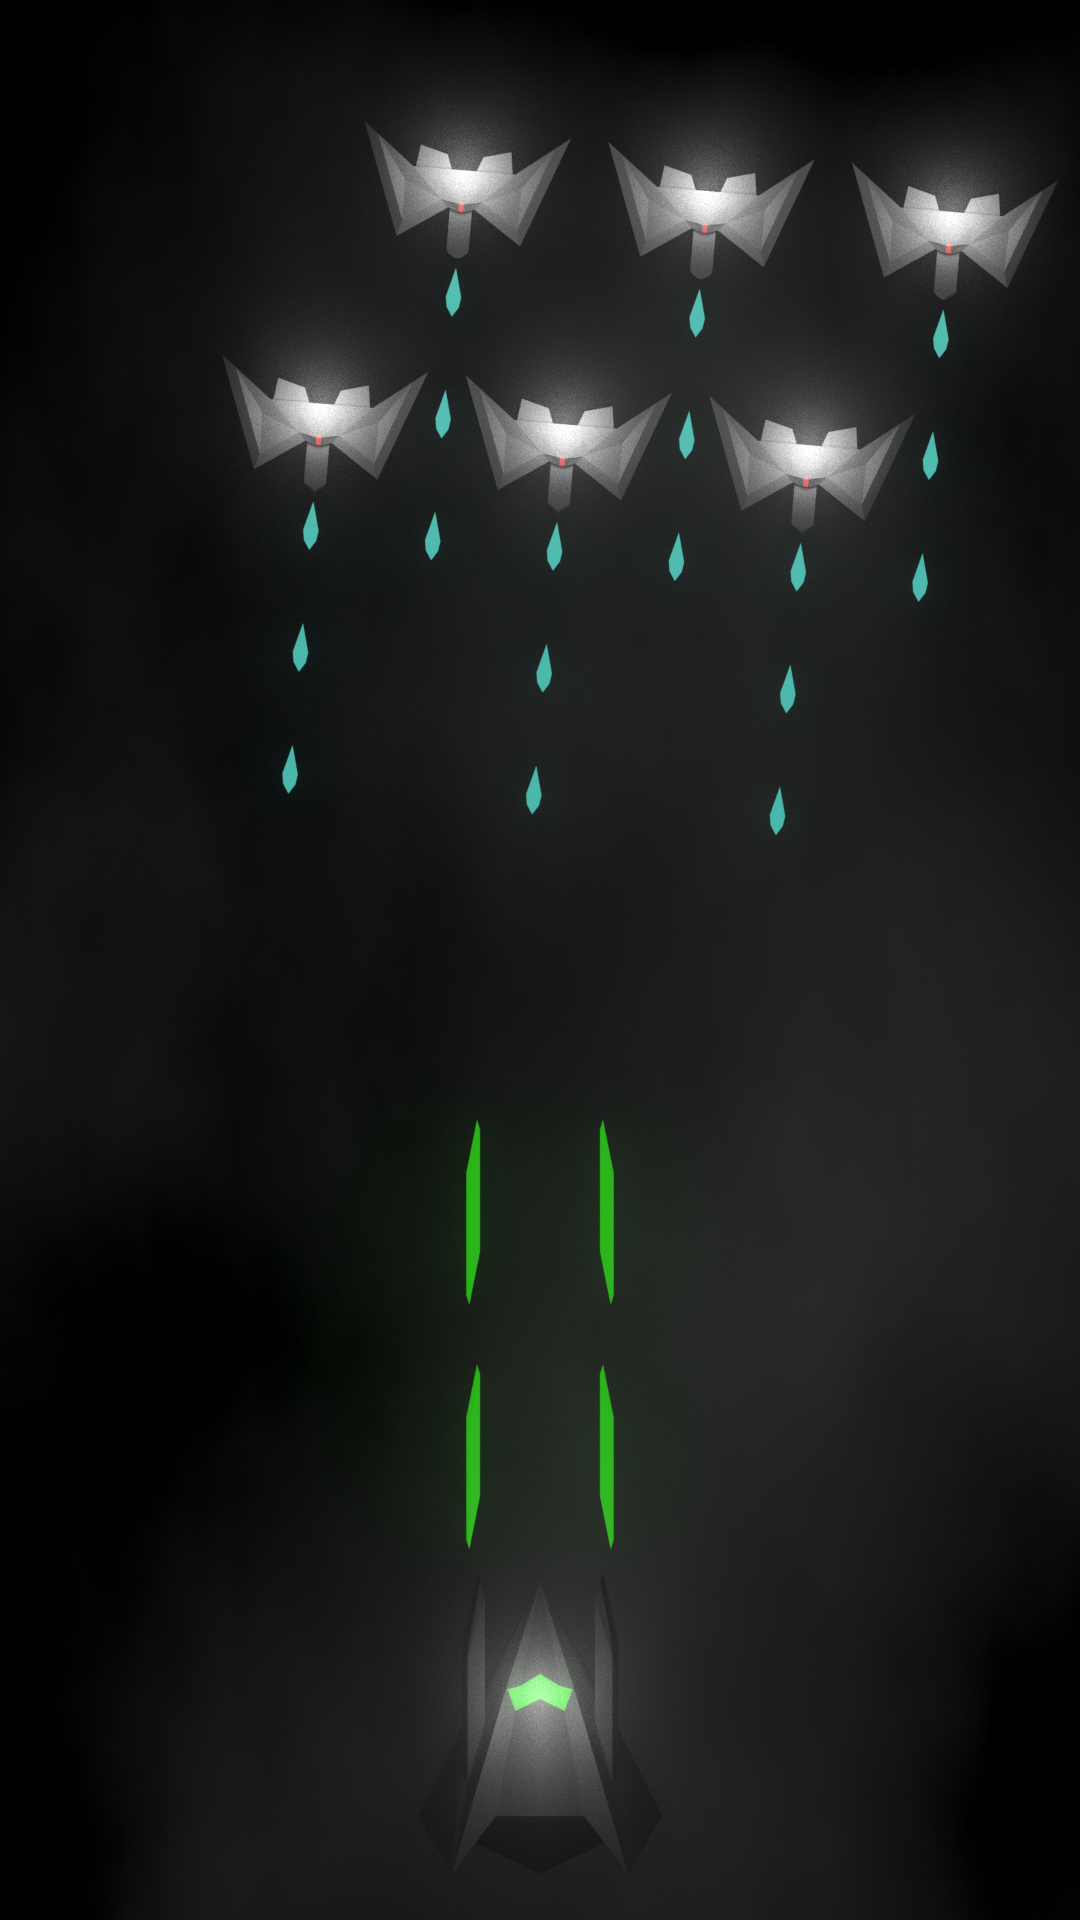
\includegraphics[width=.3\columnwidth]{mockup-01.png}
  \caption[\textit{Cybersky}]{\textit{Cybersky} Mockup Render}
\end{figure}

In terms of feel, the game is responsive in how the controls work, with a simple and versatile input system utilising the touch-screen. This is expanded upon further in section 3.3.1. With the movement relying on being responsive, the feel of the game should be fast and utilise reflexes, and this is compounded by the utilisation of particles and post-effects that enhance the visual depth to the scene.

With regards to the visual style, simplistic and yet visually detailed 3D design affords a lot of artistic freedom without much of a hardware limitation; this makes the game more accessible, and lets the environment and object design heavily impact the narrative.

\subsection{Narrative}

Summarising everything included in this document already, \emph{Cybersky} is a futuristic dystopia whereby the player controls a rogue drone (or ship) that faces off against a large automated army of drones. This world primarily revolves around a space-faring power that has taken control of 'the core worlds', a general setting for the game.

The story of the game revolves around the rogue element getting in contact with a resistance cell, discovering that the antagonist group commits atrocities and deserves to be fought against. The story doesn't conform to a standard three act structure, instead being an over-arching narrative allowing for simplistic story elements of fighting against the antagonist, or potentially an anthology of short stories that fit into the larger narrative.

\section{
  Game Mechanics
 }

\subsection{Game Rules}

Summarising what's touched upon in this document already, \emph{Cybersky} is a fixed-shooter with one dimensional or two dimensional movement, where the player shoots forward at all times. The player must acquire items to improve their abilities, and face against various enemy types, which appear at the top or sides of the screen. Bosses are high level enemies at the end of levels, which have specific abilities, phases and movesets, in which the player should learn to overcome a specific boss style to overcome it.

\subsection{Core Loops}

The core loop for \emph{Cybersky} revolves around 'stages', where difficulty steadily increases upon completion of each stage. Each stage has a gameplay or narrative focussed goal, such as "defeat the boss at the end of the level" or "find the key to [narrative element]'. On top of this, each time the player dies, their 'run' is reset, putting them back to the beginning of the stage progression. Stages follow an anthology style of storytelling, allowing for a random order of stories to keep each 'run' engaging.

To add to this, each run also progresses in difficulty, in such a way that the player doesn't get overwhelmed or find it too easy. This requires some form of balance system, whereby the player gains or loses points or unlocks to get more powerful or less powerful over time.

The permadeath nature of each run is engaging as it means that the player is disincentivised for failing a stage; they lose out on story progress, and it may be a while before they can see the story through to it's completion. Some features may be needed to keep a failed story relevant, such as a failed story queue, so that the player can catch up again without losing track. Additionally, this long-term progression should be engaging as it helps to raise the bar for skill requirement over time, keeping the game challenging.

\subsection{Control Schemes}

\subsubsection{Touch}

The game is designed for use on a mobile phone screen primarily, utilising the bottom of the screen for positioning. See Figure 2 for a wireframe.

\begin{figure}[!h]
  \centering
  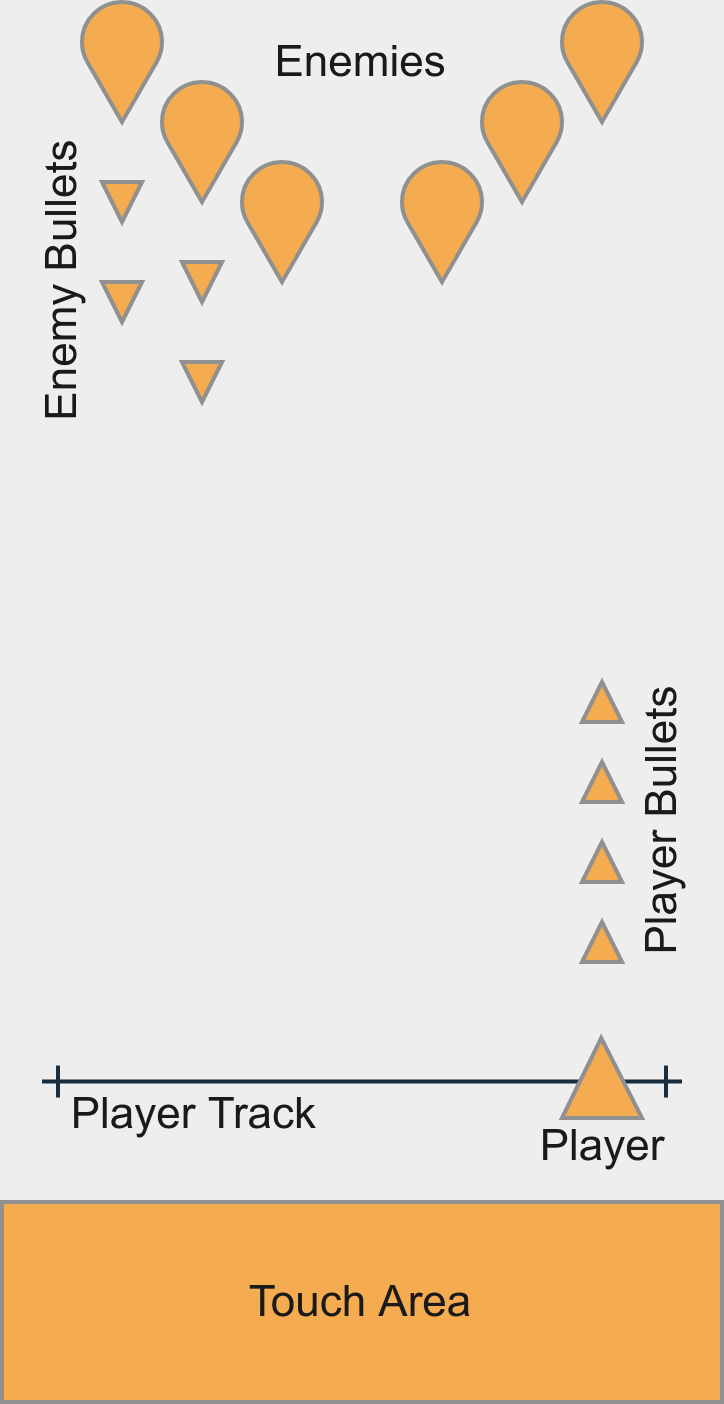
\includegraphics[width=.3\columnwidth]{concept1.png}
  \caption[\textit{Cybersky}]{\textit{Cybersky} Scene Wireframe}
\end{figure}

The proposed control method involves having an area at the bottom of the screen where the player can swipe or tap to have the ship move horizontally. Vertical movement is not planned as this may be overly complicated for the style of game. This being said, more testing is needed. The scene wireframe in Figure 2 illustrates this control method.

This method of control affects the experience in multiple ways:

\begin{itemize}
  \item The control system is accessible and simplistic, making it easy for entry level gamers to pick up and play.
  \item Additionally, the control system allows for high level players to accurately move around obstacles.
\end{itemize}

\subsubsection{Controller, Keyboard and Mouse}

This fixed-shooter style gameplay translates well to controller layout and Keyboard \& Mouse. With a controller, it's possible to control both the one-dimensional fixed-shooter style movement with the left stick, and, should it be implemented, the two dimensional movement outlined above. Keyboard \& Mouse are a little more complicated, as one of the things that keyboards are less useful for is precise positioning. Because of this, it might be useful to implement some kind of mouse control, mirroring that of the touch input.

\printbibliography

\end{document}
